% this file is called up by thesis.tex
% content in this file will be fed into the main document

%: ----------------------- name of chapter  -------------------------
\chapter{Appendix B: Serre Duality and Riemann-Roch}\label{serre_duality} % top level followed by section, subsection


%: ----------------------- paths to graphics ------------------------

% change according to folder and file names
\ifpdf
    \graphicspath{{figures/}{figures/}{figures/}}
\else
    \graphicspath{{figures/}{figures/}}
\fi

%: ----------------------- contents from here ------------------------

In this Chapter we give the statement and a proof of the \RR Theorem. As we will see, the \emph{cheap} version of the result can be easily obtained, while the complete statement heavily relies on the Serre Duality Theorem, which we prove in Section \ref{sec:Serre_duality} following the original work of Serre.\\ 
Further, in Section \ref{sec:alpha_delta} we give a motivation for the fact that the restriction map 
$$ \al:H^0(K)\to H^0(K\otimes \OD) $$ 
is, with respect to the Serre duality pairing, dual to the cohomological coboundary map 
$$\delta:H^0(D)_D\to H^1(\OX).$$

\section{Cheap Riemann-Roch}
	In this section we state and prove the \emph{cheap version} of the fundamental \RR theorem. We will be able to prove the complete version of the theorem at the end of this Appendix, exploiting Serre duality.
	\begin{namedtheo}[Cheap \RR Theorem]\label{thm:cheap_RR}
		Let $X$ be a complete curve of genus $g$, $K$ a canonical divisor and $D\in \Dd$. Then
		$$ h^0(D) - h^1(D) = \deg(D)-g+1. $$
	\end{namedtheo}
	\begin{rema}
		The \textbf{Euler characteristic} of a line bundle $L$ over a curve $X$ is defined as
		$$ \chi(L) = h^0(X,L) - h^1(X,L), $$
		so we can rewrite the statement of the \RR as
		$$ \chi(D) = \deg(D) - g + 1. $$
	\end{rema}
	\begin{proof}
		We first prove the theorem for effective divisors $D\geq 0$, proceeding by induction over $d=\deg(D)$. For $d=0$ we obtain $\OD=\OX$ and, since by definition $g=h^1(\OX)$, the formula holds trivially
		$$ h^0(\OX) - h^1(\OX) = 1-g. $$
		Now suppose the relation holds for all effective divisors with $\deg<d$. Let $D'\geq 0$ be of degree $d-1$ and set $D=D'+P$ for $P\in X$. We have a short exact sequence of quasi-coherent sheaves
		$$ \SES{\calO(D')}{\OD}{k_P}, $$
		where $k_P$ is the skyscraper sheaf at $P$ and the map ${\OD}\to{k_P}$ is the evaluation at $P$. Thus using the fact that the Euler characteristic is additive on \sess we obtain
		$$ \chi(D) = \chi(D') + 1 = (d-1-g+1) + 1 = d-g+1, $$
		as required. For the general case $D=D_1-D_2$ with $D_i$ effective of degree $d_i$ we have the \ses
		$$ \SES{\OD}{\calO(D_1)}{k^{d_2}} $$
		which easily leads to the desired result.
	\end{proof}

\section{Serre Duality Theorem}\label{sec:Serre_duality}

	This Section is based on the first chapter of the wonderful book \emph{Algebraic Groups and Class Fields} written by Serre, which appears as entry number \cite{SERRE} in our Bibliography.\\

	Even though Serre duality for curves can be derived as a consequence of Grothendieck's duality Theorem (see for instance Theorem III.7.6 of \cite{HAG}), we will give a more direct proof for the case of curves, inspired by the classical proof used by Weil. A crucial ingredient is the the ring of repartitions, which we now introduce.
	\begin{defi}
		Define $R$, the \textbf{ring of repartitions} on $X$, as the set of collections $\{r_P\}_{P\in X}$ such that $r_P\in k(X)$ for every $P\in X$ and $r_P\in \calO_{X,P}$ for all but finitely many $P\in X$. This is a very big ring, containing in particular $k(X)$, but can also be seen as a $k$-vector space.
		Further, for any divisor $D\in \Div_X$, we define $R(D)$ to be the $k$-vector subspace of $R$ consisting of those repartitions $r$ for which
		$$ v_P(r_P) + v_P(D) \geq 0, \qquad \forall P\in X. $$
	\end{defi}
	As one can easily guess, the space $R(D)$ is strictly related to the invertible sheaf $\OXD$. The following proposition will make this idea precise, but first we need an easy Lemma.
	\begin{lemm}\label{lemm:H1}
		Let $X$ be an irreducible topological space and $\uA$ a constant sheaf of abelian groups on $X$. Then
		$$ H^1(X, \uA) = 0 $$
	\end{lemm}
	\begin{proof}
		Let $\{ U_\al \}_{\al \in I}$ be an open cover of $X$ and $(g_{\alb})$ be a $1$-cocycle in $Z^1(X, \uA)$. Since $X$ is irreducible, the constant presheaf $\uA^{\presheaf}$ is already a sheaf, thus we can fix $i\in I$ and define the $0$-cochain
		$$ h_\al := g_{\al, i} \qquad \forall \al \in I. $$
		The coboundary condition on $(g_{\alb})$ implies that
		$$ \partial (h_\al) = (h_\al - h_\beta) = (g_{\al, i} + g_{i, \beta}) = (g_{\alb}) $$
		so we see that $(g_{\alb})$ is a coboundary and it is therefore trivial in $H^1(X, \uA)$.
	\end{proof}
	\begin{rema}
		A shorter proof of the above Lemma can be given in terms of Grothendieck's functorial definition of sheaf cohomology. The point is that constant sheaves on algebraic varieties are \textbf{flasque}, and these have trivial cohomology in positive degrees. See Proposition $2.5$, Chapter III.2 of \cite{HAG}.
	\end{rema}
	\begin{prop}\label{prop:h1D}
		There is a canonical isomorphism $ H^1(D) \cong \frac{R}{R(D)+k(X)} $.
	\end{prop}
	\begin{proof}
		Let $\underline{k(X)}$ denote the constant sheaf with stalks $k(X)$ and let $S$ be the cokernel of the natural inclusion $\OXD\into \underline{k(X)}$. We thus have a \ses of invertible sheaves
		$$ \SES{\OXD}{\underline{k(X)}}{S} $$
		which, since by Lemma \ref{lemm:H1} we know $H^1(\underline{k(X)})=0$, gives the following exact sequence in cohomology
		$$ 0\to H^0(D)\to k(X) \to H^0(S) \to H^1(D) \to 0. $$
		Hence we just need to show that $H^0(S) \cong R/R(D)$ to be done. In order to do so recall that, by definition of quotient sheaf, $S$ is the sheaf corresponding to the pre-sheaf $S^{\presheaf}$ with stalks at $P$ given by
		$$ S_P := \frac{k(X)}{\OXD_P} $$
		Notice, moreover, that $R/R(D)$ is the direct sum of $S_P$ over all points of $X$
		$$ R/R(D) = \bigoplus_{P\in X} S_P $$
		so it suffices to show that $H^0(S)=\bigoplus_{P\in X} S_P$ get the conclusion. To see it, pick an arbitrary $P\in X$ and consider a nonzero element of the the stalk $S_P$. Extend it to a section $s\in \Gamma(U,S)$ locally defined in a neighborhood $U$ of $P$ and observe this implies that $s$ has a pole at $P$ -- otherwise it would be zero in the stalk $S_P$. Since the locus of points where $s$ is singular is a Zariski closed subset of $X$, we can find a smaller open $U'\subset U$ containing no other singularities of $s$ apart from $P$. Hence we have $s\equiv 0$ on $U'\setminus P$, so it follows that $S^{\presheaf} = S$ is a sheaf on its own right and moreover, since $X$ is complete and any discrete compact set is finite, we see that $S$ is a direct sum of skyscraper sheaves: $S=\bigoplus_{P\in X} (i_P)_* S_P$, where $i_P:P\into X$ is the inclusion of $P$ in $X$. Therefore we find
		$$ H^0(S) = H^0\left(\bigoplus_{P\in X} (i_P)_* S_P \right) = \bigoplus_{P\in X}S_P $$
		as desired.
	\end{proof}
	\begin{defi}
		Given a divisor $D$, define $J(D) := H^1(D)^{\vee}$. 
	\end{defi}
	From the above proposition it follows that $J(D)$ is the space of linear functionals $H^1(D)\to k$ which vanish on $R(D)$ and $k(X)$. Hence it follows that $J(D)\subset J(D')$ \ABiff $D'\leq D$, and we can consider the direct system
	$$ \set{ J(D) \mid D\in \Div_X } $$
	over the directed set $\set{ \Div_X, \preceq }$, where we set $D\preceq D' \iff D' \leq D$. Then we define $J$ to be direct limit of the $J(D)$'s with respect to the above direct system which, since we are taking the limit simply over the inclusion maps, coincides with the union over all divisors $D\in \Div_X$ of the sets $J(D)$.
	\begin{rema}
		Notice that $J$ has a natural structure of vector space over $k(X)$: if $\al\in J(D)$ and $f\in H^0(E)$ then the product $f\cdot\al$ belongs to $J(D-E)\subset J$.
	\end{rema}
	We can give a very strict bound on the dimension of $J$ which will be essential to prove Serre duality. 
	\begin{prop}\label{prop:dim1}
		The dimension of $J$ as a vector space over $k(X)$ is at most $1$.
	\end{prop}
	\begin{proof}
		Suppose $\al$ and $\beta$ are two elements of $J$ which are linearly independent over $k(X)$ and notice that we can always find a divisor $D$ of degree $d$ such that $\al,\beta \in J(D)$. Further, observe that for any divisor $E$ of degree $e$ and functions $f,g \in H^0(E)$ we have
		$$ f \al \in J(D-E) \AND  g\beta \in J(D-E). $$
		The assumption that $\al$ and $\beta$ are linearly independent implies that the map
		$$ \ph: H^0(E)\times H^0(E) \to J(D-E) \qquad (f,g) \mapsto f\al + g\beta $$
		in an injection, therefore looking at the dimensions of the source and the target we deduce that
		$$ h^1(D-E) \geq 2 h^0(E) $$
		and using Theorem \ref{thm:cheap_RR} (Cheap Riemann Roch) we can rewrite the above inequality as
		$$ h^0(D-E)-(d-e) + g - 1 \geq 2(h^1(E)+e-g+1) \geq 2(e-g+1). $$
		In order to get the desired contradiction is now sufficient to notice that for any choice of $e=\deg(E) > d$ we have $h^0(D-E)=0$ and thus we get
		$$ 3g-3-d \geq e, $$
		clearly absurd due to the arbitrary of $e$.
	\end{proof}
	It is now finally the time to define the pairing that will give us Serre duality.
	\begin{defi}
		Let $A$ denote the space of Abelian differentials on $X$, and define the map
		$$ \pairing : R \times A \to k , \qquad \pair{r}{\omega} := \sum_{P\in X} \Res_P(r_P \cdot \omega) $$
		where we take as the definition of residue the one given in Chapter $7$ of \cite{SERRE}, which is purely algebraic.
	\end{defi}
	\begin{lemm}\label{lemm:pairing_properties}
		The map $\pairing$ has the following properties:
	\begin{enumerate}[(i)]
		\item $ r\in R(D),\; \w \in H^0(K-D) \implies \pair{r}{\w} = 0 $
		\item $ r\in k(X) \implies \pair{r}{\w}=0 $
		\item $ f\in k(X) \implies \pair{fr}{\w} = \pair{r}{f\w} $
	\end{enumerate}
	\end{lemm}
	\begin{proof}\mbox{}\\*
		\begin{enumerate}[(i)]
			\item Any repartition $r\in R(D)$ has singularities bounded by $D$ and any form in $\nobreak{H^0(K-D)}$ vanishes on $D$ with enough multiplicity, so their product is a regular form with no poles.
			\item An immediate application of the Residue Theorem.
			\item Follows directly from the definition: both $\pair{fr}{\w}$ and $\pair{r}{f\w} $ are equal to 
			$$ \sum_{P\in X} \Res_P(f \cdot r_P\cdot \w). $$ 
		\end{enumerate}
	\end{proof}
	As a consequence of the above lemma combined with Proposition \ref{prop:h1D} we obtain a well-defined pairing
	$$ \pairing : H^1(D) \otimes H^0(K-D) \to k $$
	and hence for every divisor $D$ we can define linear maps
	$$ \theta_D : H^0(K-D) \to J(D), \qquad \w \mapsto \pair{\bullet}{\w} $$
	which, since $A=\bigcup_{D} H^0(K-D)$, can be put together in a unique map $\theta:A\to J$.
	We are almost there, but before we can face the proof of Serre duality we need another easy fact.
	\begin{lemm}\label{lem:inj_duality}
		Let $\w\in A$ be an abelian differential. We have
		$$ \theta(\w) \in J(D) \implica \w \in H^0(K-D). $$
	\end{lemm}
	\begin{proof}
		Suppose $\w \not\in H^0(K-D)$. Then there is a point $P\in X$ such that
		$$ v_P(\w) < v_P(D), $$
		therefore -- if $\pi$ is a uniformizer at $P$ -- the repartition $r$ defined by
		$$ r_Q = 0 \quad \forall Q \neq P, \qquad r_P = \frac{1}{\pi^{v_p(\w) +1}} $$
		belongs to $R(D)$. Moreover we notice that $v_P(r_P \cdot \w) = -1$, hence we find
		$$ \pair{r}{\w} = \sum_{Q\in X} \Res_Q(r_Q \cdot \w) = \Res_P(r_P \cdot \w) \neq 0. $$
		This is a contradiction: by hypothesis $\theta(\w)\in J(D)$ so we should have $\pair{r}{\w} = 0.$ 
	\end{proof}
	We are finally ready to prove Serre duality, which, after our preparation, is actually a triviality.
	\begin{namedtheo}[Serre Duality Theorem]
		The pairing $\pairing$ is a duality and for every divisor $D$ we have 
		$$ H^0(K-D) \cong H^1(D)^{\vee} $$
	\end{namedtheo}
	\begin{proof}
		The linear map $\theta_D : H^0(K-D) \to H^1(D)^{\vee}$ is injective. Indeed if $\theta(\w) = 0$ then it belongs to $J(E)$ for every divisor $E$, so from Lemma \ref{lem:inj_duality} it follows that $\w \in H^0(K-E)$ and the arbitrariness of $E$ forces $\w=0$.\\
		For surjectivity notice that the space of Abelian differentials $A$ is $1$-dimensional over $k(X)$ and thus Proposition \ref{prop:dim1} forces $\theta:A\to J$ to be surjective. Therefore another application of Lemma \ref{lem:inj_duality} ensures that $\theta_D : H^0(K-D) \to H^1(D)^{\vee}$ is surjective, too.
	\end{proof}

\section{Duality between $\al$ and $\delta$}\label{sec:alpha_delta}

	The objective of this section is to show that, for every divisor $D\in X_d$, the maps
	$$ \delta:H^0(D_D)\to H^1(\OX) \AND \al:H^0(J)\to H^0(K_D) $$
	are dual to each other.
	To start, consider the \ses of invertible sheaves 
	$$ \SES{\OX}{\OXD}{\ODD} $$
	and apply the cohomology functor to obtain the long exact sequence of finite dimensional vector spaces
	\begin{equation}\label{eq:les1}
		0\to k \to H^0(D) \to H^0(D_D) \overset{\delta}\longrightarrow H^1(\OX) \to H^1(D) \to 0.
	\end{equation}
	Now let $D'=K-D$ be the residual of $D$, consider the \ses
	$$ \SES{D'}{K}{K_D} $$
	and apply the cohomology functor to get the exact sequence of vector spaces
	$$ 0\to H^0(D') \to H^0(K) \to H^0(K_D) \overset{\al}\longrightarrow H^1(D') \to H^0(D) \to 0. $$
	Serre duality ensures that the four outer terms of the dual sequence
	$$ 0\to H^1(K)^{\vee} \to H^1(D')^{\vee} \to H^0(K_D)^{\vee} \overset{\al^{\vee}}\longrightarrow H^0(K)^{\vee} \to H^0(D')^{\vee} \to 0. $$
	are isomorphic the the corresponding terms of $\ref{eq:les1}$. Hence, exploiting to the functoriality of the duality pairings $\theta$, we get a commutative diagram
	\begin{equation}\label{eq:diagram}
		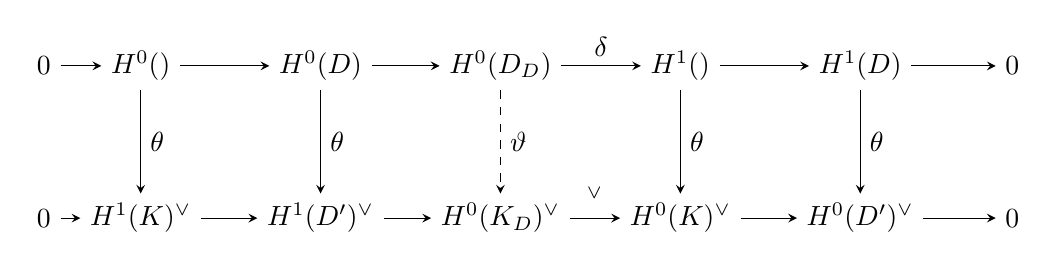
\begin{tikzpicture}[node distance=6.5em, auto]
			\node 					(01) 																{$0$};
			\node 					(A) 	[right of=01, xshift=-3em]		{$H^0(\OX)$};
			\node 					(B) 	[right of=A, xshift=-0em]			{$H^0(D)$};
			\node 					(C) 	[right of=B]									{$H^0(D_D)$};
			\node 					(D) 	[right of=C]									{$H^1(\OX)$};
		  \node 					(E) 	[right of=D]									{$H^1(D)$};
			\node 					(02) 	[right of=E, xshift=-1em]			{$0$};
			%
			\node 					(01') [below of=01, yshift=1em]		{$0$};
			\node 					(A') 	[right of=01', xshift=-3em]		{$H^1(K)^{\vee}$};
			\node 					(B') 	[right of=A', xshift=-0em]		{$H^1(D')^{\vee}$};
			\node 					(C') 	[right of=B']									{$H^0(K_D)^{\vee}$};
			\node 					(D') 	[right of=C']									{$H^0(K)^{\vee}$};
		  \node 					(E') 	[right of=D']									{$H^0(D')^{\vee}$};
			\node 					(02') [right of=E', xshift=-1em]		{$0$};
			%
		  \draw[-stealth]	(01)		to node {$\;$} 		(A);
		  \draw[-stealth]	(A)			to node {$\;$} 		(B);
		  \draw[-stealth]	(B)			to node {$\;$}	 	(C);
		  \draw[-stealth]	(C)			to node {$\delta$}(D);
		  \draw[-stealth]	(D)			to node {$\;$} 		(E);
		  \draw[-stealth]	(E)			to node {$\;$} 		(02);
		  %
		  \draw[-stealth][swap]	(01')		to node {$\;$} 		(A');
		  \draw[-stealth][swap]	(A')		to node {$\;$} 		(B');
		  \draw[-stealth][swap]	(B')		to node {$\;$}	 	(C');
		 	\draw[-stealth][]	(C')				to node {$\al^{\vee}$} 	(D');
		  \draw[-stealth][swap]	(D')		to node {$\;$} 		(E');
		  \draw[-stealth][swap]	(E')		to node {$\;$} 		(02');
			%
		  \draw[-stealth]	(A)							to node {$\theta$} 		(A');
		  \draw[-stealth]	(B)							to node {$\theta$}	 	(B');
		  \draw[-stealth, dashed]	(C)			to node {$\vartheta$} 		(C');
		  \draw[-stealth]	(D)							to node {$\theta$} 	(D');
		  \draw[-stealth]	(E)							to node {$\theta$} 		(E');
		\end{tikzpicture}
	\end{equation}
	and invoking the Five Lemma we obtain the dashed isomorphism $\vartheta$, which we use to define the perfect pairing
	$$ \pairing : H^0(D_D)\otimes H^0(K_D) \to k $$
	so that the desired duality between $\al$ and $\delta$ is a consequence of the commutativity of the above diagram. In other words for every $ v\in H^0(D_D)$ and $\w\in H^0(K_D)$ we have the formula
	\begin{equation}\label{eq:deltalpha}
		\pair{\delta v}{\w} = \pair{v}{\al \w}
	\end{equation}

	\begin{figure}[h]
		\centering
		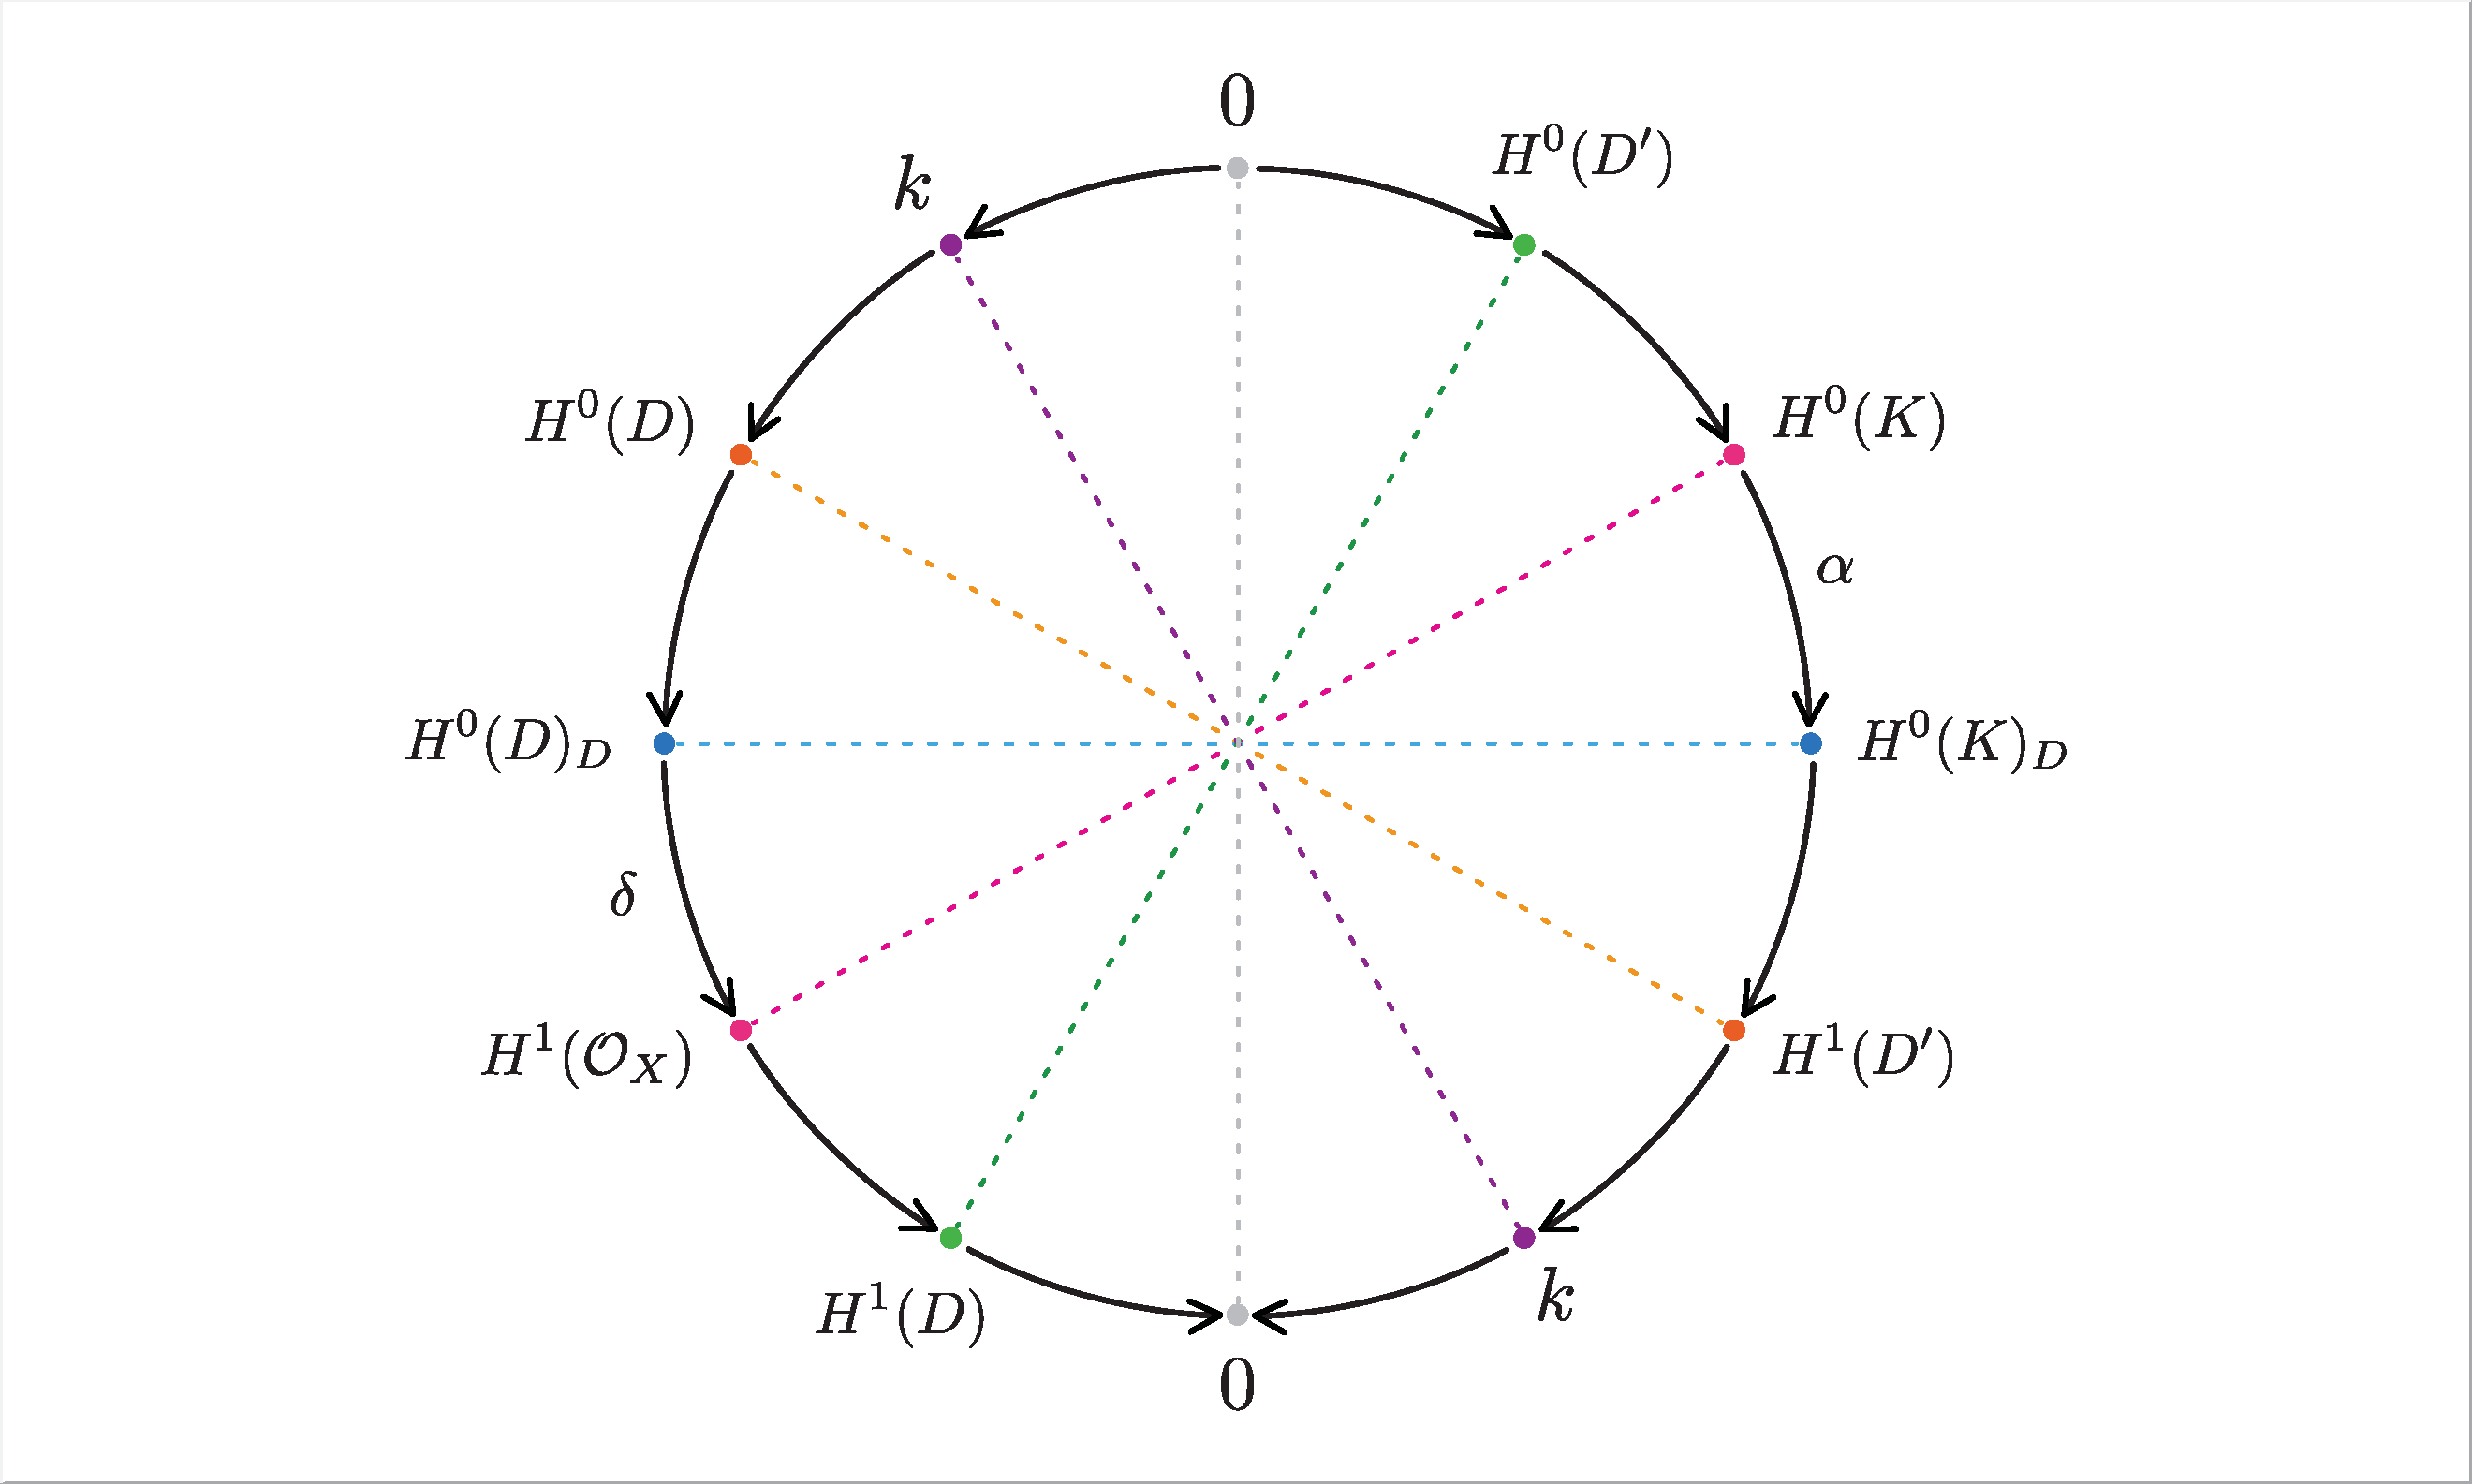
\includegraphics[width=0.9\textwidth]{Dual_Circle.pdf}
		\caption{ A more \emph{artistic} representation of the duality involved in diagram \eqref{eq:diagram} }
		\label{fig:Dual_Circle}
		\vspace{2em}
	\end{figure}


\section{Riemann-Roch Theorem}
	Using Serre duality we immediately get the final version of the theorem.
	\begin{namedtheo}[\RR Theorem]
		Let $X$ be a complete curve of genus $g$, $K$ a canonical divisor and $D\in \Dd$. Then
		\begin{equation}\label{thm:RR}
			h^0(D) - h^0(K-D) = d-g+1
		\end{equation}
	\end{namedtheo}
	Notice that, plugging-in the canonical class $K$ in the \RR formula and recalling that by definition $h^0(K) = g$, we get
	$$ \deg(K) = 2g-2 $$
	which, since $K$ is the dual of the tangent bundle, is an analogue of the Hopf index theorem for Riemann surfaces.
	
	
	
	
	
	
	
	% ---------------------------------------------------------------------------
	% ----------------------- end of thesis sub-document ------------------------


